\documentclass[10pt,twocolumn,letterpaper]{article}

\usepackage{statcourse}
\usepackage{times}
\usepackage{epsfig}
\usepackage{graphicx}
\usepackage{amsmath}
\usepackage{amssymb}
\usepackage{enumitem}
\usepackage[hyphens]{url}
\usepackage{paralist}
\usepackage{pgfplots}
\pgfplotsset{compat=1.16}
\usepackage{verbatim}
\usepackage{makecell}
% to set figures where they belong
\usepackage[section]{placeins}
%\usepackage{layouts}%

% Include other packages here, before hyperref.

% If you comment hyperref and then uncomment it, you should delete
% egpaper.aux before re-running latex.  (Or just hit 'q' on the first latex
% run, let it finish, and you should be clear).
\usepackage[breaklinks=true,bookmarks=false]{hyperref}


\statcoursefinalcopy


\setcounter{page}{1}
\begin{document}

%\currentpage
%\pagedesign



%%%%%%%%%%%%%%%%%%%%%%%%%%%%%%%%%%%%%%%%%%%%%%%%%%%%%%%%%%%%%%%
% DO NOT EDIT ANYTHING ABOVE THIS LINE
% EXCEPT IF YOU LIKE TO USE ADDITIONAL PACKAGES
%%%%%%%%%%%%%%%%%%%%%%%%%%%%%%%%%%%%%%%%%%%%%%%%%%%%%%%%%%%%%%%



%%%%%%%%% TITLE
\title{FINAL REPORT \\ diCtNN: A Dictionary-Enhanced CNN Approach \\ for Classifying Hate Speech on Twitter}


\author{Carlos Eduardo Posada\\
{\tt\small c.posada@mpp.hertie-school.org}
\and
Maximilian Kupi\thanks{These authors are sharing the project between the NLP and Python class.}\\
{\tt\small m.kupi@mpp.hertie-school.org}
\and 
Michael Bodnar\\
{\tt\small m.bodnar@mpp.hertie-school.org}
\and
Nikolas Schmidt\footnotemark[1]\\
{\tt\small n.schmidt@mpp.hertie-school.org}}

\maketitle
%\thispagestyle{empty}



% MAIN ARTICLE GOES BELOW
%%%%%%%%%%%%%%%%%%%%%%%%%%%%%%%%%%%%%%%%%%%%%%%%%%%%%%%%%%%%%%%


%%%%%%%%% ABSTRACT
\begin{abstract}
Hate speech is a growing concern, particularly on social media, and automated methods have so far been sub-par at reliably detecting it. Challenges lie in the evasive nature of hate speech, particularly in the ambiguity and fast evolution of natural language. In this paper, we propose a new multi-class classification approach, aiming to address this issue. We implement a Convolutional Neural Network (CNN) architecture and fuse a pretrained BERT word embedding with a second embedding layer based on a dictionary of hateful words. We classify a dataset of 110,748 tweets into three categories: \textit{hateful}, \textit{abusive}, and \textit{normal}. By adding the dictionary-enhanced input, we are able to increase our model's predictive power and increase the F1 macro score by seven percentage points in comparison to the simple BERT embedding.
\end{abstract}

%%%%%%%%% BODY TEXT
\section{Introduction\protect\footnote{If not further specified, all code for the model, as well as for the grid search, training and testing, was written by the authors. The code can be accessed from \href{https://github.com/MaximilianKupi/nlp-project}{this GitHub repository (clickable link)} and the documentation can be accessed from \href{https://nlp-project-documentation.readthedocs.io/en/latest/}{ readthedocs.io (clickable link)} }}\label{Section 1}

With the widespread use of social media, hateful content has become a concerning issue \cite{Costello2018PredictorsYouth}. Hateful content, such as comments on Twitter and Facebook, target individuals or groups based on ethnicity, national background, gender identity, sexual orientation, class or disability \cite[p.~130 ff.]{Jacobs2001HatePolitics}. Studies have shown that social media can serve as a propagation mechanism, and suggested that hateful online messages are predictors of real-world hate crimes \cite{Muller2017}. In order to discourage violence, social networks and other online venues have sought to remove these harmful messages from their platforms. However, their manual removal is unfeasible due to the high volume of comments in a growing number of social media venues. Thus, most recently, automatic methods have been employed.

Detecting, classifying and removing hate speech is a complex task from a technical point of view. Some of the difficulties include \cite{MacAvaney2019}:
\begin{compactitem}
    \item The lack of a common definition of hate speech, which leads to different classification criteria as well as diverging databases of hateful comments. Hate speech detection tools which are trained on these databases can thus carry biases.
    \item The nuances of natural language, such as sarcasm, sentiment and double meanings, increase the difficulty of distinguishing between hate speech and innocuous expressions.
    \item Keeping up with the lexical evolution of hate speech leads to a need to constantly update the dictionaries.
\end{compactitem}
\smallskip
Given these difficulties, the use of deep learning methods has been proposed as a novel approach to hate speech detection. However, the recently developed approaches come with certain new limitations, such as the use of user data —besides the actual text of the tweet or comment— to make the predictions, limiting the method's applicability across platforms \cite{Meyer2019ADetector}; and the difficulty to accurately discern between tweets or comments that are merely offensive and actual hate speech. To tackle these limitations, we developed diCtNN, a deep-learning classifier of hate speech in tweets. We utilise a Convolutional Neural Network (CNN) for a three-class classification problem and categorise tweets into \textit{hateful}, \textit{abusive}, and \textit{normal} tweets.

In our baseline model, the input to the CNN is a tensor of tweets, which have been cleaned and then vectorised using a pretrained BERT model. The key feature in our enhanced, final model is a dictionary approach, in which we assign a value of hatefulness to every word in each tweet, based on an established dictionary of hateful terms. The tweet-level vector of hatefulness values is then transformed into a tensor and stacked with the tensor resulting from the BERT vectorisation of each tweet, resulting in a two-dimensional input for our CNN.

Our testing results show that this enhancement improves the model's predictive power as it helps to better distinguish between \textit{hateful}, \textit{abusive}, and \textit{normal} tweets.

The next section will highlight important related work in the field of hate speech detection. Section \ref{Section 3} will outline the methods and theory employed in the development and evaluation of our diCtNN, while the section following thereafter will detail the experiments carried out and their results. Finally, the analysis section will provide a qualitative evaluation of our work. The main part of the paper will end with a conclusion. 

\section{Related Work}\label{Section 2}

The literature on hate speech detection has evolved over the past years regarding its definition, its context of occurrence, and the applied computational methods. Initially, surface-feature extractions of the text (e.g. token and character n-grams) were combined with other methods (e.g. bag of words, word generalisation or term-frequency-inverse document frequency) for classification \cite{Schmidt2017}. A variety of machine learning algorithms have been employed in past literature \cite{Nobata2016AbusiveContent}, for example support vector machines \cite{Ibrohim2019Multi-labelTwitter}. However, in recent years, neural networks have become the state of the art, in particular in combination with the use of different word-embedding techniques to represent and group text data in a vector space \cite{kim_convolutional_2014, Kshirsagar2018PredictiveTwitter, Orac}.

Research has also explored the utilisation of further characteristics of hate speech: sentiment analysis can work as a sub-approach to hate speech detection, focusing on strong negative sentiments to differentiate normal from hate speech \cite{Rodriguez2019AutomaticAnalysis, Schmidt2017, Watanabe2018HateDetection}. However, this has not improved results substantially, in particular when considering the controversy regarding legally-binding definitions of hate speech: strong negative sentiment alone does not yet constitute hate speech.

On the other hand, approaches to identify hate speech based on the presence of offensive language (rather than sentiment) have proven to have limited accuracy as well, due to the possibly innocuous use of certain offensive words \cite{hateoffensive}. One way of addressing this is to diversify the classification problem, e.g. by including a category for \textit{offensive} / \textit{abusive} content, next to \textit{hateful} and \textit{normal} content. This gives both a differentiated orientation for manual tagging as well as more nuanced basis for deep-learning classification \cite{Fortuna2019ADataset, founta2018large}.

Another way of identifying hate speech in online content is to include user data and other metadata into the analysis \cite{Mathew2019SpreadMedia, Ribeiro2018CharacterizingTwitter, Waseem2016HatefulTwitter}, with some authors even going so far as to rely solely on that type of data \cite{Miro-Llinares2018HateMicroenvironments}. In these approaches, the focus lies more on identifying hateful user accounts and environments, rather than hateful content per se. This is mostly useful in specific circumstances of real-time online interactions, where deleting chat content retroactively misses the point. An example for this are online-gaming chats, where banning users is the routine practice \cite{Stoop2019DetectingDevelop}. However, metadata collection differs across platforms and thus impedes a model's applicability to other datasets or platform environments \cite{Meyer2019ADetector}.

An alternative or additional approach is to make use of a dictionary or lexicon of hateful terms to detect hate speech. This can be done by building a dictionary of terms or phrases from a manually tagged dataset \cite{Gitari2015ADetection, Mulki2019L-HSAB:Language} or by matching content against an external dictionary. However, so far dictionaries have mostly been utilised in rule-based machine classification \cite{Martins2018} — for example, in order to select potentially hateful content (such as tweets) from a broader database of content or to assess the classification quality of crowd-sourced manual tagging \cite{hateoffensive, Mulki2019L-HSAB:Language}. To our knowledge, our approach of fusing a pretrained word embedding with a second embedding layer based on a dictionary of hateful words as input into a deep-learning architecture is a novelty in the literature.\footnote{In addition, none of the previous approaches has taken into account an ambiguity measure or offensiveness rating of hateful terms (see Section \ref{Section 3}).}

\section{Proposed Method}\label{Section 3}

To develop diCtNN, we followed a two-staged path: first, we established a CNN model architecture to solve the three-way classification problem; second, we  implemented our dictionary approach in order to enhance the input into this CNN architecture.
\paragraph{Choice of model:}
CNN architectures typically excel at computer vision as well as image and video processing, but have also shown promising results in natural language processing (NLP) and speech recognition \cite{Khan2020ANetworks}. In NLP, other architectures such as Recurrent Neural Networks (RNNs) have also been used, including Gated Recurrent Unit (GRU) and Long Short-Term Memory (LSTM) RNN architectures \cite{Adel2017}. However, in detecting hate speech, CNNs have been shown to offer distinctive advantages.

Namely, CNNs are adept at extracting features and recognising patterns from word combinations.\footnote{In contrast to this, RNNs rely on features found in sequences.} This specificity of CNNs is relevant for hate speech, where certain combinations of words occur often, while the sequence in which certain words occur is less important. Additionally, tweets are short\footnote{140 characters in the data we are using; Twitter changed the maximum character length of a tweet to 280 characters in 2017.}, which makes the capability to detect sequences in a single tweet, as is the approach of RNN alternatives, less useful for our purposes. This is especially relevant when hate speech is determined by the occurrence of specific words\footnote{This approach in understanding hate speech underpins also our further investigation methods, see remainder of this section.}, whereas modelling a longer sequence —such as done with GRU— can miss key words that determine the meaning within a sequence \cite{Yin2016}.

Furthermore, CNN architectures have been shown to be more efficient than RNN architectures, as RNNs take longer or more computing power to train \cite{Adel2017}.\footnote{While this may not be an issue in our application, as our data input is limited, striving for efficiency in use of computational power should be a matter of principle.} For these reasons, we have chosen a CNN model architecture to distinguish between \textit{hateful}, \textit{abusive}, and \textit{normal} tweets. We implemented that architecture in Python, using the PyTorch library \cite{PyTorch2019}.

\paragraph{Convolutional Neural Network:}
CNNs are a special kind of multi-layer perceptron that include additional layers called convolutional layers, in which the process of convolution occurs. In this process, a filter, which is a small matrix of weights or parameters, also called a kernel, is applied to the input data in matrix form in order to capture local correlations between points (e. g. spatial and temporal dependencies) \cite{Khan2020ANetworks}, and at the same time reduce processing complexity and time \cite{Saha2018}. In our baseline model, the input matrix and the kernel are matrices of height 1, i.e. vectors. For the implementation of our dictionary approach, however, we use 2-dimensional matrices.

During convolution, the kernel strides over the input matrix. While striding, it is matrix-multiplied with a new section of the input matrix. The results of the multiplication are summed up and after the kernel has stridden over the whole input matrix, a matrix of weighted sums is obtained. This output has reduced complexity over the input dataset and conserves the most essential features, defined by the kernel. The first layers of convolution extract low-level features of the input data, while later layers capture high-level features \cite{Saha2018}.

Padding is another characteristic of the convolution process. It consists of adding extra zero values to the input matrix, so that the kernel can cover its edges equally while striding. For our model, we performed padding before each convolution so that the convolved matrices had the same size as the input matrices and their dimensions were maintained throughout the network \cite{Saha2018}. Besides padding, other relevant hyperparamenters have been set as follows, based on the usual conventions for text classification: the size of the kernel, which defines the shape of the convolution, has been set to three; and the stride, which controls the size of the steps the kernel takes while displacing over the input matrix, has been set to one \cite{Rao2019}.

After the convolutions, the final output matrices are flattened into a vector and fed into a multi-layer perceptron, which receives the extracted features and calculates the values for final classification \cite{Newatia2019}. The loss is computed by comparing the predicted and the true labels, in our case, using a multi-class cross-entropy loss function. Finally, the weights of the kernel are adapted based on the loss through backpropagation. This is how the network "learns" \cite{Khan2020ANetworks}.

\paragraph{Enhancing vectorised input with a second dimension:}
As the key distinguishing feature in our model we enhance the vectorised input to the CNN with data derived from the Hatebase dictionary, an established dictionary of hateful terms.\footnote{Davidson et al. \cite{hateoffensive}, whose dataset makes up the smaller part of our merged dataset (~20\%), have also made use of the Hatebase dictionary to preselect tweets for manual labelling.} This addresses the common challenge of distinguishing hate speech from abusive or normal tweets.

This method is then integrated into the vectorisation process of the cleaned tweets, which is implemented with a pretrained model of BERT \cite{Devlin2018}. BERT models are bidirectionally trained, so they achieve a better sense of language context than single-directional models. For efficiency and reliability reasons, we employ the BERT-base-uncased model \cite{Rajapakse2020}. The maximum vector length is set to 120 and padded with zeros. Both processes are applied to every tweet in our dataset and the resulting tensors are stacked. In order to stack the tensors, the tensor of the hatefulness values is stretched to the length of the tensor resulting from the BERT vectorisation (see next paragraph). The resulting matrix is then used as an input for the 2D-architecture of our model, as opposed to the 1D-architecture which we used in our baseline model, where the input consists only of the BERT-vectorised word embedding.

The additional input of the dictionary is designed to more clearly classify tweets in which unambiguously hateful terms are used. This innovative element distinguishes our architecture from other approaches, detailed in Section~\ref{Section 2}. Furthermore, our approach relies solely on text feature analysis and uses no metadata, user-specific or otherwise, thus classifying only content, not users, as hateful. 

\paragraph{Convolution - how the model learns based on both inputs:}\label{Subsection 1.3} 
The following explanation is based on the master documentation of PyTorch \cite{PyTorch2019}.

To understand the way we train our model to make it able to predict the hatefulness of tweets, we have to take a closer look at the mathematical concepts used, and follow one tweet through preprocessing and training. As discussed above, we use two different approaches and combine them in our model, as can be seen in Figure \ref{fig:vectorization}. While the BERT vectoriser produces a vector of a length that depends on the tokenisation of BERT, our dictionary approach uses another method of tokenisation to identify full nouns without lemmatisation and other changes.\footnote{We ran different models with and without lemmatisation of the terms in the Hatebase dictionary and found that lemmatisation did not add to the predictive power, as many terms in the dictionary were not recognised and therefore not lemmatised in the first place.} This produces two vectors, which can be of different lengths. To put the value that results from the hate dictionary analysis into the vicinity of the actual BERT-encoded word, we stretch the dictionary-derived vector with linear interpolation. This way, the length of both vectors match, and the hate dictionary evaluation will be close to its BERT embedding.

\begin{figure}[h]
    \begin{center}
        \includegraphics[scale=0.9]{writing/02_final-report-latex/figures/processing-regular.pdf}
        \caption{Preprocessing of tweets and combination of BERT vectorisation with hate dictionary approach (own visualisation)}
        \label{fig:vectorization}
    \end{center}
\end{figure}

To harmonise the input of our CNN over all the tweets, we pad the resulting matrix with zeros at the end until the matrix is of length $120$ (see Figure~\ref{fig:padding1}).

\begin{figure}[h]
    \begin{center}
        \includegraphics[width=6.5cm,keepaspectratio]{writing/02_final-report-latex/figures/processing-padding.pdf}
        \caption{Padding of the preprocessed matrix to harmonise the data set for the CNN (own visualisation)}
        \label{fig:padding1}
    \end{center}
\end{figure}

As discussed above, a convolution is used to combine multiple input values with different weights attached to them to an output value. We call the object that contains all the weights used in the calculation a kernel, which is defined through the weight matrix $[w_{ij}]=W\in\mathbb{R}^{3 \times 3}$.

The first layer gets a 2D matrix $X\in\mathbb{R}^{2\times 120}$ of length $120$ and height $2$ as input. Based on the settings for kernel size, stride, and dilation the kernel is applied to a sub-matrix $\tilde{X}=[x_{ij}]$ of input matrix $X$.

We can define the application of the kernel to one sub-matrix mathematically as a function that takes the sub-matrix $\tilde{X}$ and a matrix of weights $W$ to calculate a weighted sum, i.e. the convolution:
$$f:\mathbb{R}^{3\times 3}\times\mathbb{R}^{3 \times 3}\rightarrow \mathbb{R}, \hspace{0.3cm}(\tilde{X},W)\mapsto \sum_{i,j=1}^3 w_{ij} x_{ij} =:y_* $$

The actual learning of the model is based on the weights that we train. A weight matrix is convoluted at every layer with sub-matrices of the input matrix to create a new output matrix. The matrix is padded again with zeros to ensure that the convolution with the matrix is not reducing the overall size of the matrix that is moving through the neural network. In Figure \ref{fig:convolution}, a matrix with height $2$ is padded with one row of zeros to allow a kernel of size $3$ to reduce the matrix to an output of height $2$ again.

\begin{figure}[h]
    \begin{center}
        \includegraphics[width=6.5cm,keepaspectratio]{writing/02_final-report-latex/figures/processing-convolution.pdf}
        \caption{Convolution of weight matrix $W=[w_{ij}]$ with submatrix of padded input matrix to produce output matrix $Y=[y_{ij}]$ (own visualisation)}
        \label{fig:convolution}
    \end{center}
\end{figure}

Each neuron in our network comes with its own weight matrix. The initial weights for these weight matrices $W$ are generated randomly with a uniform distribution of values. All neurons in the first layer get the same input vector but will produce different convolutions due to the randomness of the weights.
If all weights would be equal then the back-propagation algorithm that tweaks the weights after each training step would have to change all of them or choose randomly which one to adjust because all would have the same effect. Randomisation of the weights takes this decision from the algorithm by "breaking symmetry" in the network \cite[p.~297]{Goodfellow-et-al-2016}. Thus, the randomisation is the precondition for the network to learn.

PyTorch calculates the range of values from which it can draw from randomly by considering the amount of input values and the kernel size.
The possible weights must be in the range $(-\sqrt{k},+\sqrt{k})$, where $k$ is defined through the kernel size and the input channels.

If we look at all the convolutions happening in order to produce the output of one neuron, we can see that an individual input value is included in multiple weighted sums.
The choice of $k$ ensures that neurons with different kernel size and/or input channel amount produce convolutions that are in the same numerical range. This happens through a kind of normalisation in the definition of $k$.
Each neuron in the neural network has its own weights and draws them randomly from a uniform random distribution, e.g. $w_{11},w_{12},w_{21} \in\mathcal{U}(-\sqrt{k},+\sqrt{k})$ like in Figure \ref{fig:initweights}.
\begin{figure}[h]
    \begin{center}
        \includegraphics[width=5cm,keepaspectratio]{writing/02_final-report-latex/figures/processing-weights.pdf}
        \caption{Random initialisation of kernel weights (own visualisation)}
        \label{fig:initweights}
    \end{center}
\end{figure}

In each neuron the convolution is repeated for all sub-matrices of the vector (or only a part of it depending on kernel size, stride and dilation). This results in multiple matrix multiplication per neuron which applies the kernel to each sub-vector and outputs one matrix with the result of all the associated convolutions (see Figure \ref{fig:convolution}).

Finally a bias $B$ is added to the convolution. The initial bias $B$ is drawn randomly from the same uniform distribution as before:  $\mathcal{U}(-\sqrt{k},+\sqrt{k})$.

While the weights $W$ determine the focus of the calculations, the bias $B$ directly influences the result of the activation function of the neuron. If the activation function is a Sigmoid function (see Figure \ref{fig:sigmoid}) then e.g. a simple shift to the left (negative $b$) could reduce the whole neuron output to zero and thus make the information covered in the convolutions irrelevant for the network. The bias puts some neurons' activation threshold lower and some higher in the beginning, and allows the network to focus on the relevant information. As was mentioned above in relation to the weights, the initial randomisation of the bias allows the network to learn what to focus on.

\begin{figure}[ht]
    \begin{center}
        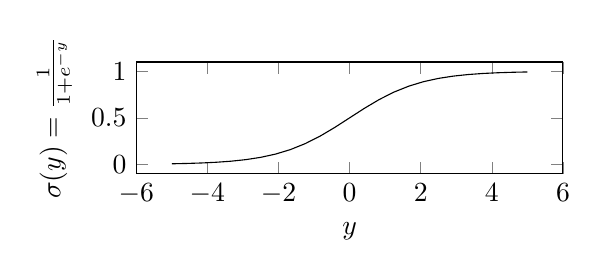
\begin{tikzpicture}
          \begin{axis}[
            height=3cm,
            width=7cm,
            ymax=1.1,
            ymin=-0.1,
            xlabel=$y$,
            ylabel={$\sigma(y) = \frac{1}{1+e^{-y}}$}
          ] 
            \addplot[mark=none] {1/(1+e^(-x))};
          \end{axis}
        \end{tikzpicture}
        \caption{Sigmoid function (own visualisation)}
        \label{fig:sigmoid}
    \end{center}
\end{figure}

The weights and the bias are adjusted depending on the loss after each training step through the back-propagation algorithm. In conclusion, the stacking of the two vectors in conjunction with the here described mathematical operations of a CNN network will ensure that our model draws on both – the BERT-vectorised as well as the dictionary vectorised – inputs to learn.

\paragraph{Data preprocessing:} The tweets were preprocessed in order to remove noise before the vectorisation process \cite{Lata2018}. The text was transformed to lower case, and symbols\footnote{As BERT also vectorises punctuation, we employed one cleaning version where standard sentence punctuation (!?.,) was preserved, and tested this version against the one with full symbol removal (see Section \ref{Section 4}).}, whitespaces and standalone digits were removed. Tweet-specific traits, i.e. URLs, mentions, reserved words, emojis and smileys were also removed.\footnote{Using the tweet-preprocessor program from Said Özcan: \url{https://pypi.org/project/tweet-preprocessor/}.} The content of hashtags (i.e. "idiots" in the case of "\#idiots") was preserved.

\paragraph{Model architecture:}
We use a CNN architecture with four hidden layers (three convolutional and one final linear layer) as well as a ReLU activation function, and batch normalisation after each convolution.\footnote{Modelled after a CNN template from:  \url{https://adventuresinmachinelearning.com/convolutional-neural-networks-tutorial-in-pytorch/}} The initial number of channels is set to one, as we input one matrix per tweet. The output channels of the first, second, and third CNN layer have been set to 16, 32, and 64, respectively. As discussed above, we apply a kernel of size three with one row of zero padding and stride of one to preserve the feature dimensions throughout the network \cite{Dumoulin2016AGT}. The out features of the final linear layer have been set to three in order to match the three classes of the tweet annotation. For a visualisation of the model architecture see Figure~\ref{fig: architecture} on the next page. 

\begin{figure*}[!h]
    \begin{center}
        \includegraphics[width=17cm,keepaspectratio]{writing/02_final-report-latex/figures/model_architecture.pdf}
        \caption{The employed CNN model architecture (including padding - own visualisation)}\label{fig: architecture}
    \end{center}
\end{figure*}

\section{Experiments}\label{Section 4}
\paragraph{Data:} We use the following two datasets for our classification task:
\begin{compactitem}
    \item The dataset from Davidson et al. \cite{hateoffensive}, which is composed of 25,000 tweets that have been preselected using the crowd-sourced \textit{Hatebase} hate speech keyword lexicon (see Section~\ref{Section 3}) and manually labeled using the crowd-sourcing platform CrowdFlower
    \item The dataset from Founta et al. \cite{founta2018large}, which comprises 100,000 manually annotated tweets (again using CrowdFlower) whose annotation has been checked for statistical robustness by the authors 
\end{compactitem}
The datasets have the following labelling categories:
\begin{compactitem}
    \item Davidson et al.: \textit{hate\_speech}, \textit{offensive\_language}, \textit{neither}
    \item Founta et al.: \textit{hateful}, \textit{abusive}, \textit{normal}, \textit{spam}
\end{compactitem}
Since our focus does not lie on spam detection, we decided to delete all tweets in this category from the second dataset. Next, following the definitions of Founta et al. \cite{founta2018large}, according to which offensive and abusive language are two very similar categories, we decided to merge both datasets. The benefits of doing so are a more balanced dataset\footnote{Both original datasets had a significant class imbalance between all three classes, while the resulting dataset is more balanced – at least between the \textit{normal}, and \textit{abusive} class (see Figure~\ref{fig:counts}).} as well as an increased sample size for the \textit{hate} class, which was highly underrepresented in both datasets. Since the resulting dataset, composed of 110,748 tweets, was still rather unbalanced with respect to the \textit{hate} category (see Figure~\ref{fig:counts}), we used a stratified shuffle split, to finally divide our dataset into training (70\%), validation (15\%), and test set (15\%), while ensuring that the classes would be distributed equally amongst all splits. 
\begin{figure}[ht]
    \begin{center}
        \includegraphics[width=8cm,keepaspectratio]{writing/01_midterm-report-latex/figures/dataset_merging.pdf}
        \caption{Counts for the respective classes in the datasets}
        \label{fig:counts}
    \end{center}
\end{figure}

\paragraph{Software:} For coding and local testing we used Microsoft's  \href{https://code.visualstudio.com/}{Visual Studio Code}, and employed \href{https://github.com/}{GitHub} to share and document the code. The project was coded and deployed in the programming language Python (Version 3.7) \cite{VanRossum1995}.

\paragraph{Hardware:} To train our models on GPUs we used \href{https://colab.research.google.com/}{Google Colab}. 
Furthermore, we executed computing intensive tasks, e.g. the vectorisation of the tweets, on a remote EC2 instance running Jupyter Lab on Amazon Web Services (AWS) through \href{https://aws.amazon.com/sagemaker/}{AWS SageMaker}.

\paragraph{Evaluation method:} As a first metric to evaluate whether the model was training correctly, we observed the evolution of the accuracy on the training and validation set over the training epochs. Furthermore, the decrease of the training and validation loss over the epochs was used as an indication for the model's convergence and generalisability. However, since accuracy tends to be highly misleading due to the class imbalance of the dataset, we further paid particular attention to the F1 macro score. Finally, in order to visualise and evaluate precision and recall of the three classes in an intuitive manner, we used confusion matrix plots.

\paragraph{Experimental details:} %How you ran your experiments (e.g. model configurations, learning rate, training time, etc.)
To determine the best hyperparameters for our CNN model architecture, we made use of a grid search. We specified the following variables for the grid search:

\begin{compactitem}
    \item optimizer type (Adam, RMSprop, and SGD)
    \item learning rate (0.0001, 0.001, 0.01)
    \item whether to use a sampler in the data loader or class weights in the loss function to balance the dataset during training\footnote{In case the class weights were used, the shuffle mode in the data loader was automatically set to true in order to ensure more robust training.}
    \item whether or not to use a scheduler to decrease the learning rate (factor 0.1) based on the performance of the F1 macro score
\end{compactitem}
During grid search we trained each model in the simple 1D version (without our diCtNN preprocessing approach) for 45 epochs with a batch size of 16. We then considered the results from the best epoch with respect to the F1 macro score. Based on the results from the grid search, the best hyperparameters were selected and the simple 1D version as well as the 2D version with diCtNN preprocessing was trained for 90 epochs respectively. Furthermore, we also trained the models on a second dataset where standard sentence punctuation has not been removed.\footnote{i.e. ".",  ",",  "?",  "!" .} Figure~\ref{fig:f1} shows the F1 macro score plots for the 1D and 2D model on the dataset including standard sentence punctuation.\footnote{The loss and accuracy plots can be found in the \href{Appendix}{Appendix}.} As can be seen, the 2D model has a steeper and higher learning curve; however it also starts overfitting at around forty epochs. After this final training routine, the best performing 1D and 2D models in terms of F1 macro score have been tested on the testing set, to compare the two approaches and ensure their generalisability. 

\begin{figure}[h!]
    \begin{center}
        \begin{tabular}{c}
        1D Model with BERT Preprocessing \\
        \includegraphics[width=8cm,keepaspectratio]{writing/02_final-report-latex/figures/f1_1D_Model_27_90epochs_wp.pdf} \\
        \\
        2D Model with additional diCtNN Preprocessing \\
        \includegraphics[width=8cm,keepaspectratio]{writing/02_final-report-latex/figures/f1_diCtNN_Model_27_90epochs_wp.pdf}
        \end{tabular}
    \caption{F1 macro score plot of the 1D and 2D model over 90 epochs}
    \label{fig:f1}
    \end{center}
\end{figure}

\paragraph{Results:} 
%Report the quantitative results that you have found so far. Use a table or plot to compare multiple results and compare against baselines.
The best model from the grid search turned out to have the following specifications: Adam optimizer, 0.01 learning rate, class weights in the loss function, and a deactivated scheduler. After retraining the 1D and 2D model for 90 epochs, the trainings on the dataset which still contained sentence punctuation outperformed the ones with full symbol removal. For the 1D model the highest score was yielded in epoch 29, for the diCtNN 2D model in epoch 36 respectively. Testing these models on the testing set yielded the following results (see Table~\ref{tab: classification report}). 

\begin{table}[ht]
\begin{center}
\begin{tabular}{r c c c c}
\multicolumn{5}{c}{1D Model with BERT Preprocessing} \\
& Precision & Recall & F1 Score \\
             \textit{hateful
}   & 0.21    &  0.26 &     0.23 \\
             \textit{abusive}& 0.69    &  0.62 &     0.66  \\
             \textit{normal} & 0.73    &  0.76 &     0.74  \\
 Accuracy  &         &       &     0.68   \\
Macro Avg   &0.54    &  0.55 &     0.54  \\
 Micro Avg  &0.68    &  0.68 &     0.68   \\
\\
 \multicolumn{5}{c}{2D Model with additional diCtNN Preprocessing} \\
&Precision & Recall & F1 Score \\
                 \textit{hateful} &0.31   &   0.30  &    0.30\\
             \textit{abusive}&  0.76   &   0.68  &    0.72 \\
             \textit{normal} &  0.77   &   0.83  &    0.80  \\
 Accuracy  &         &         &    0.74  \\
Macro Avg  &  0.61   &   0.61  &    0.61 \\
 Micro Avg  & 0.74   &   0.74  &    0.74  
\end{tabular}
\end{center}
\caption{Classification report of the best 1D model and 2D model}
\label{tab: classification report}
\end{table}

As can be seen, our diCtNN outperformed the simple 1D model on all levels. Yet, in comparison to Davidson et al. \cite{hateoffensive}, who trained classifiers on the smaller subset of our data and yielded an overall precision, recall and F1 score of above 0.90 with their best models, our performance metrics seem rather low.\footnote{Since they framed their problem as a one-versus-rest problem, these score are best compared to the micro F1 score.} However, since Davidson et al. did not apply a deep neural network architecture for classification – instead they used linear support vector machines and logistic regression – and framed the problem as a one-versus-rest classification, which significantly reduced the problem of class imbalance, these results are hardly comparable.

\section{Analysis}\label{Section 5}
In order to check our basic assumption that \textit{hateful} tweets contain more hateful words and hence mapping them on a second dimension would potentially improve the model performance, we calculated the average hatefulness of each tweet per label based on the respective tensor entries of the second dimension (see Table~\ref{tab: hatescores}). As can be seen in the table, the average hate scores are distributed as expected. 

\begin{table}[ht]
\begin{center}
\begin{tabular}{r c c c }
& \textit{hateful} & \textit{
abusive} & \textit{normal} \\
Average Hate Score     &126.28&      89.91&       56.26\\
\end{tabular}
\end{center}
\caption{Average total hate scores of tweets per label}
\label{tab: hatescores}
\end{table}

Comparing the two models' performance on the test set based on the confusion matrix (see Figure~\ref{fig:confusion}) shows that our approach outperforms the simple 1D BERT model: All percentages on the top left to bottom right diagonal increase, while all other percentages decrease. Hence, precision and recall for distinguishing between \textit{hateful}, \textit{abusive} and \textit{normal} speech on twitter can be increased by applying our innovative diCtNN approach. 

\begin{figure}[h!]
    \begin{center}
        \begin{tabular}{c}
        1D Model with BERT Preprocessing \\
        \includegraphics[width=8cm,keepaspectratio]{writing/02_final-report-latex/figures/confusion_matrix_testing_CNN_experiment_1D_FINAL.pdf} \\
        \\
        2D Model with additional diCtNN Preprocessing \\
        \includegraphics[width=8cm,keepaspectratio]{writing/02_final-report-latex/figures/confusion_matrix_testing_CNN_experiment_2D_FINAL.pdf}
        \end{tabular}
    \caption{Confusion matrix of the 1D and the 2D model}
    \label{fig:confusion}
    \end{center}
\end{figure}

However, as can be seen by the relatively high percentage in the top right of the matrix, both models still have problems with wrongly classifying hate speech as normal speech. Generally, this can partly be due to the specifically high class imbalance between those two classes: Since \textit{hateful} is the smallest class, it is likely, just by random chance, that any algorithm mistakenly classifies a tweet from this class to belong to the biggest class, which is the \textit{normal} class. However, taking a closer look at the \textit{hateful} tweets which our diCtNN approach wrongly classified as \textit{normal} revealed four further potential explanations: First, some tweets are labelled as \textit{hateful}, but contain no usual \textit{hateful} words, so our algorithm did not catch them. Example:

\begin{quote}
\textit{"@user1 @user2 @realDonaldTrump The only solution to not having children gassed to death is to bring down entire Syrian govt"}\footnote{Any occurrence of abusive or hateful content in this paper is for exemplary purpose only and not meant to offend anyone.}
\end{quote}
Second, some normal tweets have actually been wrongly labelled as \textit{hateful}, as they, for example, only report about hate. Exemplary tweet: 
\begin{quote}
"\textit{I just watched a video with a crowd of white ppl shouting nigga \& going crazy to songs about black men killing each other \& it made me so sad}".\footnote{Interesting to note about this specific case is that our algorithm classified it "correctly in real terms" as normal. This might be the case because the hatefulness in the second dimension of our input matrix functions as a magnifying for the algorithm to know which words in the first dimension it should look at. And in this specific case the hate terms identified by the algorithm ('\textit{crowd}', '\textit{white}', \& '\textit{nigga}') are rather regularly used 'hate' words that are not particularly distinct for hate tweets, so the algorithm classified the tweet as normal. Of course, this rather speculative explanation would have to be further investigated using explainable AI approaches that actually show where the CNN is looking.}
\end{quote}
Third, our dictionary-preprocessing algorithm does not catch all the \textit{hateful} words in some tweets. This might be due to the fact, that in the implemented version it does not match bi-grams, or the word simply is not contained in the \textit{Hatebase} dictionary – as this generally only includes nouns. Example tweet that fulfils both these conditions: 
\begin{quote}
"\textit{\#AmericaIsOverParty I TOLD YALL CAUCASIAN, COUSIN FUCKING, INCEST FUCKS TO NOT VOTE FOR TRUMP NOW LOOK WHAT YALL DID}"
\end{quote}
Fourth, and finally, the definition of hate speech, and which tweets fall under this definition, is still an ongoing debate \cite{Dorris2020TowardsLanguage}, and sometimes also a matter of political perspective or even potentially diverging realities as can be seen in the first example tweet.

\section{Conclusion}\label{Section 6}
We have shown that enriching BERT vectorisation with content-based embedding via a dictionary approach can substantially improve a CNN model's performance in distinguishing between \textit{hateful}, \textit{abusive}, and \textit{normal} tweets.\footnote{If deployed for real-time hate speech detection on Twitter, the dictionary from \textit{Hatebase} would need to be vetted for consistency with the platform guidelines and regularly updated.} Future research might further improve our approach (e.g. implementing bi-gram matching of hateful terms or testing other neural network model architectures such as LSTMs or GRUs), and apply it to other datasets or compare it to state-of-the-art results of other approaches. With adaptation, this approach could also be applied to other text classification problems, provided that a widely accepted dictionary of terms for the specific domain exists.\footnote{We have coded our preprocessing functions with maximum flexibility for different specifications so as to ease such further application.}

\section{Acknowledgements}\label{Section 7}
The authors would like to express their gratitude to Antigoni M. Founta of \cite{founta2018large} for granting access to the complete dataset of their study.

\section{Contributions}\label{Section 8}
\\
\\
\noindent \textbf{E. Posada} was responsible for doing the cleaning of tweets, and coding the testing method of the model. He also provided the visualisation of the architecture and part of the code documentation.
\\
\\
\textbf{M. Kupi} was responsible for dealing with the datasets as well as for setting up the grid search and the tracking of relevant metrics during training and testing. He also oversaw the training and testing routine, visualised and analysed the model results, and did most part of the code documentation.
\\
\\
\textbf{M. Bodnar} coded the class to setup the neural network as well as the methods for the vectorisation of tweets in 1D and 2D. He also provided visualisations for mathematical aspects of the network.
\\
\\
\textbf{N. Schmidt} was responsible for developing, setting up and implementing the dictionary approach (in multiple versions) as well as the testing of (mainly preprocessing) functions. He also contributed to the vectorisation and cleaning functions.
    
\section{Sharing project}
M. Kupi and N. Schmidt share the project between the NLP and Python class.

%\newpage
{\small
\bibliographystyle{ieee}
\bibliography{writing/references.bib}
}
\newpage
\section{Appendix}\label{Appendix}
%
\begin{figure}[h]
    \begin{center}
        \begin{tabular}{c}
        1D Model with BERT Preprocessing \\
        \includegraphics[width=8cm,keepaspectratio]{writing/02_final-report-latex/figures/loss_1D_Model_27_90epochs_wp.pdf} \\
        \\
        2D Model with additional diCtNN Preprocessing \\
        \includegraphics[width=8cm,keepaspectratio]{writing/02_final-report-latex/figures/loss_diCtNN_Model_27_90epochs_wp.pdf}
        \end{tabular}
    \caption{Loss plot of the 1D and 2D model over 90 epochs}
    \label{fig:loss}
    \end{center}
\end{figure}
%
%
\begin{figure}[h]
    \begin{center}
        \begin{tabular}{c}
        1D Model with BERT Preprocessing \\
        \includegraphics[width=8cm,keepaspectratio]{writing/02_final-report-latex/figures/accuracy_1D_Model_27_90epochs_wp.pdf} \\
        \\
        2D Model with additional diCtNN Preprocessing \\
        \includegraphics[width=8cm,keepaspectratio]{writing/02_final-report-latex/figures/accuracy_diCtNN_Model_27_90epochs_wp.pdf}
        \end{tabular}
    \caption{Accuracy plot of the 1D and 2D model over 90 epochs}
    \label{fig:accuracy}
    \end{center}
\end{figure}

\end{document}